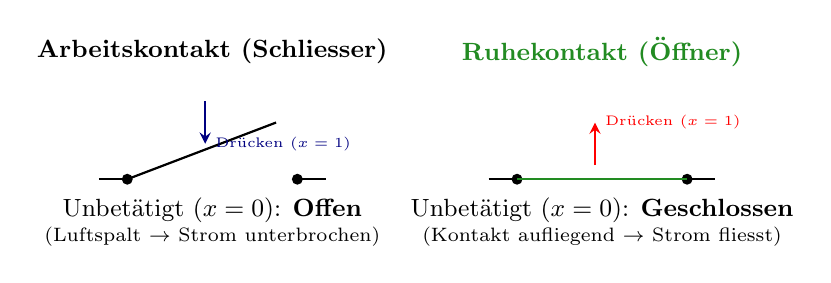
\begin{tikzpicture}[scale=0.9, >=stealth]
    % --- Arbeitskontakt (Schliesser) ---
    \begin{scope}[shift={(0,0)}]
        \node[font=\small\bfseries] at (1.2, 1.8) {Arbeitskontakt (Schliesser)};
        % Anschlüsse und Festkontakte
        \draw[thick] (-0.4,0) -- (0,0); \fill (0,0) circle (2.2pt);
        \draw[thick] (2.4,0) -- (2.8,0); \fill (2.4,0) circle (2.2pt);

        % Schalterhebel offen
        \draw[thick] (0,0) -- (2.1, 0.8);
        \draw[->, thick, NavyBlue] (1.1, 1.1) -- (1.1, 0.5) node[right, font=\tiny] {Drücken ($x=1$)};

        \node[font=\small, align=center] at (1.2, -0.6) {Unbetätigt ($x=0$): \textbf{Offen}\\[-2pt]{\scriptsize(Luftspalt $\rightarrow$ Strom unterbrochen)}};
    \end{scope}

    % --- Ruhekontakt (Öffner) ---
    \begin{scope}[shift={(5.5,0)}]
        \node[font=\small\bfseries, ForestGreen] at (1.2, 1.8) {Ruhekontakt (Öffner)};
        % Anschlüsse und Festkontakte
        \draw[thick] (-0.4,0) -- (0,0); \fill (0,0) circle (2.2pt);
        \draw[thick] (2.4,0) -- (2.8,0); \fill (2.4,0) circle (2.2pt);

        % Schalterhebel aufliegend (geschlossen)
        \draw[thick, ForestGreen] (0,0) -- (2.4,0);
        \draw[->, thick, Red] (1.1, 0.2) -- (1.1, 0.8) node[right, font=\tiny] {Drücken ($x=1$)};

        \node[font=\small, align=center] at (1.2, -0.6) {Unbetätigt ($x=0$): \textbf{Geschlossen}\\[-2pt]{\scriptsize(Kontakt aufliegend $\rightarrow$ Strom fliesst)}};
    \end{scope}
\end{tikzpicture}
